This chapter will walk you through the creation of a simple interaction
manager, which you can either create yourself, or just follow by looking at the
playground system named \texttt{ChatCat}¸ which is placed in the
\texttt{examples} folder. More complex examples are planned to be added soon.

The simplest version of an interaction manager analyses natural language
coming from the user, and generates natural language and gestures for the robot
resp. its virtual replacement, an avatar. Generation is based on incoming
stimuli, like speech or text input, or high-level action requests coming from
some strategic planning component, or any other sensor input, if available.

In this tutorial, we will create a very simple example system that has a
database representation of itself and the user it will interact with. It can
greet the user, ask for his/her name and say goodbye.

\section{Setting up the Basic Data Structures}
\label{sec:example-hfc}

A dialogue system aiming for social interaction does need some kind of memory
representation. Therefore, the first step of building your dialogue manager
with \vonda will be to set up your basic data structures in the form of an OWL
ontology. The RDF database serves two purposes: it contains 1) the data
structure definitions of the data that is used in the dialogue system, like a
\texttt{User} class and the properties that are associated with it, and 2) the
(dynamic) data objects, which are created or extended on-the-fly when the
dialogue system is running. The advantage of using and RDF store for the data
structure specifications lies in its flexibility. Extending or changing them is
easy, which is important since your system will be evolving and becoming more
and more elaborate.

For the specification of dialogue acts, we recommend that you use the dialogue
act hierarchy provided in
\texttt{examples/chatcat/src/main/resources/ontology/dialogue.nt}, which is
based on the ISO standard DIT++ hierarchy, as well as two \texttt{default}
files which are necessary for basic OWL functionality in HFC.

\subsection{Creating N-Triples Files}

%use Protege or another tool of your choice to create OWL/RDF file;
%example here: with Protege
HFC currently loads data only from files in the \texttt{N-Triples} format. The
majority of RDF software packages works with the more common RDF/XML format,
which can be automatically translated with a simple shell script that is
provided with the example (\texttt{examples/chatcat/ntcreate.sh}). This script
uses Raptor \citep{raptor}, which is provided for example in the
\texttt{raptor2-utils} \texttt{.deb} package. This tutorial uses screenshots
from Protégé \citep{Protege}, which we used for the creation of the basic
ontology, but you can just use your favourite RDF/OWL IDE.

First, create a new file that includes an RDF class \texttt{Agent}, and two
subclasses of this class, \texttt{Robot} and \texttt{Human}. After that, create
a (functional) data type predicate \texttt{name} for the class \texttt{Agent}
with the range \texttt{xsd:string}.

\begin{figure}[htb]
  \center
  \begin{minipage}{0.45\textwidth}
    \centering
    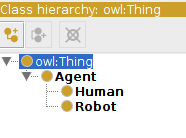
\includegraphics[width=0.6\textwidth]{Images/doc_protege.png}
  \end{minipage}\hfill
  \begin{minipage}{0.45\textwidth}
    \centering
    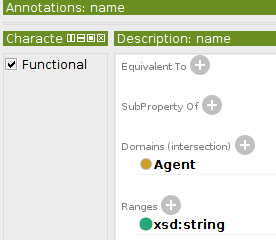
\includegraphics[width=0.6\textwidth]{Images/doc_protege2.png}
  \end{minipage}
\end{figure}

As we do not know the user a priori, we will have the system create an instance
for him/her at run-time. However, we know our robot in advance, so we create an
instance of the class Robot and name it \textit{Robert}, and then convert the
new ontology using Raptor to \texttt{N-Triples} (i.e., with the
\texttt{ntcreate.sh} script). Now, a HFC configuration file (currently in
\texttt{.ini} format) must be created, as described in the next section.

\textbf{Important:} If you are using Prot\'eg\'e, you should save the file in
RDF/XML Syntax; the script will not work properly otherwise.

\subsection{Creating a HFC Configuration File}

%Explain how multiple ontologies can be put together here; explain PersistencyFile, mention what [Namespaces] is about
The ontology files loaded into a HFC instance, and which reasoning rules are
applied, are specified in a configuration file in \texttt{.ini} format. It
also contains various settings for HFC parameters. Figure~\ref{fig:ini} shows
the config file used for the \texttt{chatcat} example. In the following, we
will explain the sections of the config file in detail.

\begin{figure} [htb]
\small%
\begin{verbatim}
[Settings]
#minNoArgs=3
#maxNoArgs=4
#noAtoms=100000
#noTuples=500000
# This file store tuples created or changed during run-time
PersistencyFile=tuples.nt
Encoding=UTF-8

[Namespaces]
# namespaces for XSD, RDF, RDFS, and OWL are already defined
dial = http://www.dfki.de/lt/onto/common/dialogue.owl#
cat = http://www.semanticweb.org/anna/ontologies/2018/3/chatcat#

# instead, you can also load one or more namespace files
#default.ns

[Tuples]
# the axiomatic triples for OWL-Horst w/ EQ reduction
default.eqred.nt

[Tuples]
dialogue.nt
# the name for the base ontology
chatcat.nt

[Rules]
# we need special rules for transaction time (mixture of triples/quadruples)
default.eqred.quads.rdl
\end{verbatim}
\caption{An exemplary HFC \texttt{config.ini} file}
\label{fig:ini}
\end{figure}



\paragraph{[Settings]}

For most applications concerning dialogue management, it is important to
specify a \emph{PersistencyFile} to save the data between two runs of the
system. This file can be put in any location, it will be created automatically
in the specified place. If your application relies on inter-session memory,
you probably don't want it to reside in some temporary directory. All new
information that your dialogue system enters into the database will be
collected here. The persistency file can also be used to find out which tuples
have been created, i.e, for on-line and post-mortem debugging. If you want to
wipe the memory of your system, simply delete this file.

\paragraph{[Namespaces]}

This section contains abbreviations for ontology namespaces. The abbreviation
\texttt{dial} in figure \ref{fig:ini}, allows to refer to
\texttt{<http://www.dfki.de/lt/onto/common/dialogue.owl\#Accept>} using
\texttt{<dial:Accept>} instead, for example in queries to the database. As
you can see, we included a shortcut for our chatcat ontology here.

\paragraph{[Tuples]}

Here all ontology files have to be listed that should be loaded into the
knowledge base on start-up. The persistency file, if you have specified one,
will be loaded automatically. You should also include the file
\texttt{dialogue.nt} which, as previously mentioned, contains the
specifications of the dialogue acts usually used by the \vonda framework.

\paragraph{[Rules]}

This specifies the set of rules that HFC uses for OWL reasoning. Currently, the
file \texttt{default.eqred.quads.rdl} is required for proper operation of
\vonda, since it relies on the so-called \emph{transaction time}
representation, which allows to keep a (possibly) infinite memory, while still
preserving a monotonic RDF store, i.e., only adding and never deleting
tuples. This representation uses quadruples, where the forth element is the
timestamp when the tuple was added to the store. For tuples with infinite
resp. universal validity, the timestamp should be set to zero. For further
information, please refer to the documentation of HFC.

\section{Setting up the Basic Java Classes}

First, the project's abstract (Java) ``agent'' class has to be implemented,
which must be a subclass of \texttt{de.dfki.mlt.rudimant.agent.Agent}, a class
in the run-time library of \vonda. Furthermore, you will need an implementation
of \texttt{de.dfki.mlt.rudimant.agent.CommunicationHub}. To see an example of
what these could contain, take a look in the source folder of \texttt{ChatCat}.

The two most important things here are that there is an active connection to a
database (as an instance of \texttt{RdfProxy}) and that you have an instance of
the beforementioned \vonda \texttt{Agent} wrapper implementation in your
client. Of course this code can not compile until you build your first rule
file, i.e., your \vonda Agent. Then, a \texttt{main} has to create an instance
of your client and is started using the \texttt{startListening()} method.

We recommend to have a look at the classes of the ChatCat system as a base for
your own system and extend it. It comes you with a very simple GUI to enter
text or dialogue acts which you can use to test your first dialogue steps.

\section{Connecting NLU and Generation Components}

%examplary here: srgs for NLU and cplan for generation
Basically, you can connect any NLU and NLG components to your project that are
able to create or, respectively, process dialogue acts of the format that
\vonda provides (cfg. \ref{sec:caret}).

For the sake of simplicity, this example uses SRGS to build a primitive NLU and
cplan\footnote{https://github.com/bkiefer/cplan} to create natural language out of the dialogue acts the agent outputs.

\section{First Interaction Rules}

Now that the basics have been arranged, we are set up for writing our first
dialogue management rules. First we want to react to the user greeting the
system, what we expect to be happening on startup. In the SRGS file
(\small\texttt{src/main/resources/grammars/srgs/chatcat.xml}), we defined that
an utterance of the user like ''Hello'' will be parsed as the dialogue act
\texttt{InitialGreeting}, with the proposition \texttt{Greet}. We now can
define a rule reacting to this utterance:

\begin{lstlisting}
greet_back:
  if (lastDA() <= #InitialGreeting(Greet)) {
    user = new Human;
    if (! saidInSession(#Greeting()) {
      propose("greet_back") {
        emitDA(#ReturnGreeting(Greet));
      }
    }
    lastDAprocessed();
  }
\end{lstlisting}

This will create a new instance of the RDF class \texttt{Human} we defined when
setting up the ontology, storing it in a global variable \texttt{user} that in
our case has been defined in the ChatAgent and will be present during the whole
conversation. The check \texttt{!~saidInSession(\#Greeting)} currently doesn't
seem to make sense, why this is necessary will be obvious when we have
completed the example. This test already shows an important property of the
system: \texttt{Greeting} is the superclass of \texttt{InitialGreeting} and
\texttt{ReturnGreeting} in the DIT++ ontology, and the function will return
\texttt{true}, no matter what type of greeting we gave, since it tests for
\texttt{subsumption}, like the comparison operators \texttt{<=} and \texttt{<}
that work on dialoge act arguments that we use in the next rule example. More
details about how to exploit this functionality will be given in section
\ref{sec:dialogueacts}

After greeting, we want to find out the user's name. We thus define a rule as
follows:

\begin{lstlisting}
ask_for_name:
  if (!user.name && !(myLastDA() <= #WHQuestion(Name))) {
    propose("ask_name") {
      emitDA(#WHQuestion(Name));
    }
    lastDAprocessed();
  }
\end{lstlisting}

And once we got the answer from the user, we can store this knowledge in the
database:

\begin{lstlisting}
remember_name:
  if (lastDA() <= #Inform(Name)) {
    user.name = lastDA().what;
    lastDAprocessed();
  }
\end{lstlisting}

We currently don't have a person detector, so we assume that someone's here
when the system is started. To make sure the conversation starts even if the
user doesn't start with a greeting, we use a \emph{timeout} ot implement a
system greeting after some time.

\begin{lstlisting}
timeout("robot_starts", 4000) {
 start_conversation:
  if (! (receivedInSession(#Greeting(top)) || saidInSession(#Greeting(top)))) {
    propose("robot_greets") {
      tod = Date.timeOfDay();
      emitDA(#InitialGreeting(Greet, when={tod}));
    }
  }
}
\end{lstlisting}
\todo[inline]{Explain the timeOfDay code, and that a Java import and an entry in
  ChatAgent is necessary to obtain compilable code}

These are enough rules to start a conversation, so let's compile and try out
the new dialogue system.

\section{Specifying how to Compile and Run your Project}

Now that we have implemented our first rules, we need to compile them. In the
\texttt{bin} directory of you \vonda installation is a script \texttt{vondac}
that will use you compilation config file to compile your project. The most
convenient way to use it is either to establish a softlink in a directory that
is already in your \texttt{PATH} or to add \vonda's \texttt{bin} directory to
it.

The compile.yml should contain the following parameters:\\

\begin{tabular}{ll}
  \texttt{inputFile} & Relative to the current location, where is the
                       top-level rule file?\\
  \texttt{outputDirectory} & Relative to the current location, where should the compiled classes go?\\
  \texttt{wrapperClass} & The name of your abstract Java Agent, including
                          package prefix\\
  \texttt{ontologyFile} &The path to your ontology \texttt{.ini}, relative to the current location\\
  \texttt{rootPackage} &The topmost package to put the compiled Java classes in\\
  \texttt{failOnError} &If \texttt{true} to exits compilation on any
                         encountered type errors\footnote{Note that although
                         \vonda's type checking is becoming more and more
                         elaborate and reliable, it is by no means complete. In
                         some cases, setting this switch to true might make
                         your project uncompilable although when compiling it
                         ignoring the type errors results in a perfectly sound
                         Java project.}, otherwise continues\\
\end{tabular}\\

Since the compile and the runtime phase of \vonda need different information,
e.g., the run-time phase needs NLU and NLG components, there is a second
\texttt{yaml} file for the run-time phase containing the following
specifications (This is the example from ChatCat):

\begin{verbatim}
ontologyFile:       src/main/resources/ontology/chatcat.ini
NLG:
eng:
mapperProject:      src/main/resources/grammars/cplanner/allrules-mapper
generationProject:  src/main/resources/grammars/cplanner/allrules
NLU:
eng:
class:              de.dfki.chatcat.SrgsParser
grammar:            src/main/resources/grammars/srgs/chatcat.xml
\end{verbatim}

This configuration can be used to start your compiled system by passing it to
the init method of \texttt{Agent}, allowing for easier configuration of these
modules, also in multi-language settings. You can as well put all information
into one \texttt{yaml} file, using it for run time and compile time, since the
irrelevant configuration keys will be ignored.

\subsection{Resolving Name Ambiguities} \label{sec:nsAmbigue}

As you might have noticed whilst looking at chatcat.yml, there is another
parameter used in the compile configuration of our example project:

\begin{verbatim}
nameToURI:
Agent: "<cat:Agent>"

nameToClass:
Date: de.dfki.chatcat.util.Date
\end{verbatim}

When trying to compile without the first two lines, you will find that \vonda
produces the warning \begin{small}'' \texttt{base name Agent can be one of
    <http://www.semanticweb.org/anna/ontologies/2018/3/chatcat\#Agent>,
    <dial:Agent>, please resolve manually.}''
\end{small}.

This is the compiler telling us that when defining the RDF class \texttt{Agent}
in the database step, we actually redefined an existing class. \vonda warns us
about this and urges us to resolve this ambiguity. Thus, we could either rename
our class, or explicitly state which namespace should be accessed whenever the
class \texttt{Agent} is used. \texttt{nameToURI} can be used to do the latter.
You can also use this functionality to remap RDF class names: \vonda will
always map the name on the left to the class URI provided on the right.

The second specification serves to resolve type checks in favour of Java
instead of RDF classes. The fully specified name is currently not used, but
might be used in later versions to generate Java \texttt{import} statements.

% The second specification tells us the \texttt{Date} class' fully specified
% name. This example does not help a lot by itself, but is more relevant if you
% want to use your own support classes providing functionality that is easier
% to implement in Java than in \vonda code. Together with the right field and
% method specifications, this can massively support the type checker. We will
% look into this more closely in section~\ref{sec:support}.

\if0
Natural language dialogue systems are becoming more and more popular, be it as
virtual assistants such as Siri or Cortana, as Chat Bots on websites providing
customer support, or as interface in human-robot interactions in areas ranging
from Industry 4.0 \citep{schwartz2016hybrid} over social human-robot-interaction
\citep{alize2010} to disaster response \citep{kruijff2015tradr}.

A central component of most systems is the \emph{dialogue manager}, which
controls the (possibly multi-modal) reactions based on sensory input and the
current system state. The existing frameworks to implement dialogue management
components roughly fall into two big groups, those that use symbolic
information or automata to specify the dialogue flow (IrisTK
\citep{2012iristk}, RavenClaw \citep{bohus2009ravenclaw}, Visual SceneMaker
\citep{gebhard2012visual}), and those that mostly use statistical methods
(PyDial \cite{ultes2017pydial}, Alex \citep{jurvcivcek2014alex}). Somewhat in
between these is OpenDial \citep{lison2015developing}, which builds on
probabilistic rules and a Bayesian Network.

When building dialogue components for robotic systems or in-car assistants, the system
needs to take into account \emph{various} system inputs, first and foremost the
user utterances, but also other sensoric input that may influence the dialogue,
such as information from computer vision, gaze detection, or even body and
environment sensors for cognitive load estimation.

The integration and handling of the different sources such that all data is
easily accessible to the dialogue management is by no means trivial. Most
frameworks use plug-ins that directly interface to the dialogue core. The
multi-modal dialogue platform SiAM-dp \citep{nesselrath2014siam}
addresses this in a more fundamental way using a modeling approach that allows
to share variables or objects between different modules.

In the application domain of social robotic assistants, it is vital to be able
to maintain a relationship with the user over a longer time period. This requires a long-term
memory which can be used in the dialogue system to exhibit familiarity with the
user in various aspects, like personal preferences, but also common knowledge
about past conversations or events, ranging over multiple sessions.

In the following, we will describe \vonda, an open-source framework to
implement dialogue strategies. It follows the information state/update
tradition \citep{traum2003information}
%DR Traum, S Larsson. The information state approach to dialogue management. In: Current and new directions in discourse and dialogue, 2003, pp.  325-353. Kluwer.
combining a rule-based approach with statistical selection, although in a
different way than OpenDial. \vonda specifically targets the following design
goals to support the system requirements described before:

\begin{itemize}
  \addtolength{\itemsep}{-.6\itemsep}
\item Flexible and uniform specification of dialogue semantics, knowledge and
  data structures
\item Scalable, efficient, and easily accessible storage of interaction history
  and other data, resulting in a large information state
\item Readable and compact rule specifications, facilitating access to the
  underlying RDF database, with the full power of a programming language
\item Transparent access to Java classes for simple integration with the host
  system
\end{itemize}
\fi

%%% Local Variables:
%%% mode: latex
%%% TeX-master: "userguide"
%%% End:
